\section{Aufgabe 17}
\label{sec:Aufgabe17}

\subsection*{a)}
Für den Datensatz aus Tabelle \ref{tab:data} wird ein binärer Entscheidungsbaum aufgestellt. Bei den Attributen $Wind$ und $Soccer$, werden die Werte $0$ und $1$ als $False$ bzw. $True$ interpretiert.
Die Entropie der Wurzel des Baumes bestimmt sich über die Formel
\begin{equation}
H(Soccer)= S = -\sum_.i p_.i\cdot log_.2(p_.i)
\end{equation}
mit den Wahrscheinlichkeiten
\begin{align*}
p_.{Soccer = True} &= \frac{9}{14}\\
p_.{Soccer = False} &= \frac{5}{14}
\end{align*}
zu $S\approx 0,9403$

\begin{table}
	\centering
	\caption{Datensatz zur Erzeugung eines binären Entscheidungsbaumes, ob Fußball gespielt werden sollte oder nicht.}
	\label{tab:tabData}
	\sisetup{table-format=1.2}
	\begin{tabular}{S[table-format=2.1]S[table-format=1.0]S[table-format=2.0]S[table-format=1.0]S[table-format=1.0]}
		\toprule
		{$Temperature/\si{\celsius}$} & {$Weather$} & {$Humidity/\si{\percent}$} & {$Wind$} & {$Soccer$} \\
		\midrule
		29.4 & 2 & 85 & 0 & 0 \\
		26.7 & 2 & 90 & 1 & 0 \\
		28.3 & 1 & 78 & 0 & 1 \\
		21.1 & 0 & 96 & 0 & 1 \\
		20.0 & 0 & 80 & 0 & 1 \\
		18.3 & 0 & 70 & 1 & 0 \\
		17.8 & 1 & 65 & 1 & 1 \\
		22.2 & 2 & 95 & 0 & 0 \\
		20.6 & 2 & 70 & 0 & 1 \\
		23.9 & 0 & 80 & 0 & 1 \\
		23.9 & 2 & 70 & 1 & 1 \\
		22.2 & 1 & 90 & 1 & 1 \\
		27.2 & 1 & 75 & 0 & 1 \\
		21.7 & 0 & 80 & 1 & 0 \\
		\bottomrule
	\end{tabular}

	\label{tab:data}
\end{table}

\subsection*{b)}
Der Informationsgewinn bei einem Schnitt des Attributes $Wind$ berechnet sich nach der Formel
\begin{align*}
IG(Wind,Soccer) &= H(Soccer) - H(Soccer|Wind)\\
&= S + p_.{Wind = True} H(Soccer|Wind = True )+ p_.{Wind = False} H(Soccer|Wind = False)\text{.}
\end{align*}	
Mit den Wahrscheinlichkeiten
\begin{align*}
p_.{Wind = True} &= \frac{3}{7}\\
p_.{Wind = False} &= \frac{4}{7}\\
p_.{Soccer = True|Wind = True} &= \frac{1}{2}\\
p_.{Soccer = True|Wind = False} &= \frac{3}{4}\\
p_.{Soccer = False|Wind = True} &= \frac{1}{2}\\
p_.{Soccer = False|Wind = False} &= \frac{1}{4}
\end{align*}
ergibt sich so $IG(Wind,Soccer)\approx 0,0481$

\subsection*{c)}
Im Python-Script werden die Plots für den Informationsgewinn bei verschiedenen Schnitten der Attribute erzeugt, die in den Abbildungen \ref{fig:temp} bis \ref{fig:weather} zu sehen sind.
Für das Attribut $Weather$ wurde noch ein weiterer Schnitt betrachtet, bei dem der Wert $1$, also normales Wetter, von den beiden anderen Möglichkeiten getrennt wurde.
\begin{figure}
\includegraphics[width=0.8\textwidth]{build/temp.pdf}
\caption{Informationsgewinn bei verschiedenen Schnitten für die Temperatur.}\label{fig:temp}
\includegraphics[width=0.8\textwidth]{build/humidity.pdf}
\caption{Informationsgewinn bei verschiedenen Schnitten für die Luftfeuchtugkeit.}\label{fig:hum}
\end{figure}
\newpage
\begin{figure}
\includegraphics[width=0.8\textwidth]{build/weather.pdf}
\caption{Informationsgewinn bei verschiedenen Schnitten für das Wetter.}\label{fig:weather}
\end{figure}

\subsection*{d)}
\noindent An der Ausgabe
\begin{figure}
\centering
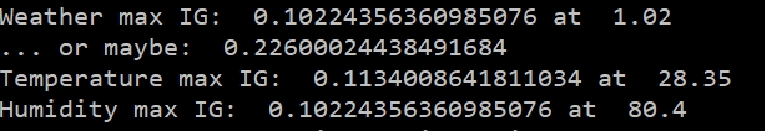
\includegraphics[width = 0.9\textwidth]{content/tables/out.pdf}
\end{figure}
\noindent lässt sich erkennen, dass die bestmögliche Trennung der Daten durch das Wetter und mit dem eben beschriebenen Schnitt generiert wird.

%Æ♣♥•☻◘♠